% Options for packages loaded elsewhere
\PassOptionsToPackage{unicode}{hyperref}
\PassOptionsToPackage{hyphens}{url}
\PassOptionsToPackage{dvipsnames,svgnames,x11names}{xcolor}
%
\documentclass[
  letterpaper,
  DIV=11,
  numbers=noendperiod]{scrartcl}

\usepackage{amsmath,amssymb}
\usepackage{iftex}
\ifPDFTeX
  \usepackage[T1]{fontenc}
  \usepackage[utf8]{inputenc}
  \usepackage{textcomp} % provide euro and other symbols
\else % if luatex or xetex
  \usepackage{unicode-math}
  \defaultfontfeatures{Scale=MatchLowercase}
  \defaultfontfeatures[\rmfamily]{Ligatures=TeX,Scale=1}
\fi
\usepackage{lmodern}
\ifPDFTeX\else  
    % xetex/luatex font selection
\fi
% Use upquote if available, for straight quotes in verbatim environments
\IfFileExists{upquote.sty}{\usepackage{upquote}}{}
\IfFileExists{microtype.sty}{% use microtype if available
  \usepackage[]{microtype}
  \UseMicrotypeSet[protrusion]{basicmath} % disable protrusion for tt fonts
}{}
\makeatletter
\@ifundefined{KOMAClassName}{% if non-KOMA class
  \IfFileExists{parskip.sty}{%
    \usepackage{parskip}
  }{% else
    \setlength{\parindent}{0pt}
    \setlength{\parskip}{6pt plus 2pt minus 1pt}}
}{% if KOMA class
  \KOMAoptions{parskip=half}}
\makeatother
\usepackage{xcolor}
\setlength{\emergencystretch}{3em} % prevent overfull lines
\setcounter{secnumdepth}{5}
% Make \paragraph and \subparagraph free-standing
\ifx\paragraph\undefined\else
  \let\oldparagraph\paragraph
  \renewcommand{\paragraph}[1]{\oldparagraph{#1}\mbox{}}
\fi
\ifx\subparagraph\undefined\else
  \let\oldsubparagraph\subparagraph
  \renewcommand{\subparagraph}[1]{\oldsubparagraph{#1}\mbox{}}
\fi

\usepackage{color}
\usepackage{fancyvrb}
\newcommand{\VerbBar}{|}
\newcommand{\VERB}{\Verb[commandchars=\\\{\}]}
\DefineVerbatimEnvironment{Highlighting}{Verbatim}{commandchars=\\\{\}}
% Add ',fontsize=\small' for more characters per line
\usepackage{framed}
\definecolor{shadecolor}{RGB}{241,243,245}
\newenvironment{Shaded}{\begin{snugshade}}{\end{snugshade}}
\newcommand{\AlertTok}[1]{\textcolor[rgb]{0.68,0.00,0.00}{#1}}
\newcommand{\AnnotationTok}[1]{\textcolor[rgb]{0.37,0.37,0.37}{#1}}
\newcommand{\AttributeTok}[1]{\textcolor[rgb]{0.40,0.45,0.13}{#1}}
\newcommand{\BaseNTok}[1]{\textcolor[rgb]{0.68,0.00,0.00}{#1}}
\newcommand{\BuiltInTok}[1]{\textcolor[rgb]{0.00,0.23,0.31}{#1}}
\newcommand{\CharTok}[1]{\textcolor[rgb]{0.13,0.47,0.30}{#1}}
\newcommand{\CommentTok}[1]{\textcolor[rgb]{0.37,0.37,0.37}{#1}}
\newcommand{\CommentVarTok}[1]{\textcolor[rgb]{0.37,0.37,0.37}{\textit{#1}}}
\newcommand{\ConstantTok}[1]{\textcolor[rgb]{0.56,0.35,0.01}{#1}}
\newcommand{\ControlFlowTok}[1]{\textcolor[rgb]{0.00,0.23,0.31}{#1}}
\newcommand{\DataTypeTok}[1]{\textcolor[rgb]{0.68,0.00,0.00}{#1}}
\newcommand{\DecValTok}[1]{\textcolor[rgb]{0.68,0.00,0.00}{#1}}
\newcommand{\DocumentationTok}[1]{\textcolor[rgb]{0.37,0.37,0.37}{\textit{#1}}}
\newcommand{\ErrorTok}[1]{\textcolor[rgb]{0.68,0.00,0.00}{#1}}
\newcommand{\ExtensionTok}[1]{\textcolor[rgb]{0.00,0.23,0.31}{#1}}
\newcommand{\FloatTok}[1]{\textcolor[rgb]{0.68,0.00,0.00}{#1}}
\newcommand{\FunctionTok}[1]{\textcolor[rgb]{0.28,0.35,0.67}{#1}}
\newcommand{\ImportTok}[1]{\textcolor[rgb]{0.00,0.46,0.62}{#1}}
\newcommand{\InformationTok}[1]{\textcolor[rgb]{0.37,0.37,0.37}{#1}}
\newcommand{\KeywordTok}[1]{\textcolor[rgb]{0.00,0.23,0.31}{#1}}
\newcommand{\NormalTok}[1]{\textcolor[rgb]{0.00,0.23,0.31}{#1}}
\newcommand{\OperatorTok}[1]{\textcolor[rgb]{0.37,0.37,0.37}{#1}}
\newcommand{\OtherTok}[1]{\textcolor[rgb]{0.00,0.23,0.31}{#1}}
\newcommand{\PreprocessorTok}[1]{\textcolor[rgb]{0.68,0.00,0.00}{#1}}
\newcommand{\RegionMarkerTok}[1]{\textcolor[rgb]{0.00,0.23,0.31}{#1}}
\newcommand{\SpecialCharTok}[1]{\textcolor[rgb]{0.37,0.37,0.37}{#1}}
\newcommand{\SpecialStringTok}[1]{\textcolor[rgb]{0.13,0.47,0.30}{#1}}
\newcommand{\StringTok}[1]{\textcolor[rgb]{0.13,0.47,0.30}{#1}}
\newcommand{\VariableTok}[1]{\textcolor[rgb]{0.07,0.07,0.07}{#1}}
\newcommand{\VerbatimStringTok}[1]{\textcolor[rgb]{0.13,0.47,0.30}{#1}}
\newcommand{\WarningTok}[1]{\textcolor[rgb]{0.37,0.37,0.37}{\textit{#1}}}

\providecommand{\tightlist}{%
  \setlength{\itemsep}{0pt}\setlength{\parskip}{0pt}}\usepackage{longtable,booktabs,array}
\usepackage{calc} % for calculating minipage widths
% Correct order of tables after \paragraph or \subparagraph
\usepackage{etoolbox}
\makeatletter
\patchcmd\longtable{\par}{\if@noskipsec\mbox{}\fi\par}{}{}
\makeatother
% Allow footnotes in longtable head/foot
\IfFileExists{footnotehyper.sty}{\usepackage{footnotehyper}}{\usepackage{footnote}}
\makesavenoteenv{longtable}
\usepackage{graphicx}
\makeatletter
\def\maxwidth{\ifdim\Gin@nat@width>\linewidth\linewidth\else\Gin@nat@width\fi}
\def\maxheight{\ifdim\Gin@nat@height>\textheight\textheight\else\Gin@nat@height\fi}
\makeatother
% Scale images if necessary, so that they will not overflow the page
% margins by default, and it is still possible to overwrite the defaults
% using explicit options in \includegraphics[width, height, ...]{}
\setkeys{Gin}{width=\maxwidth,height=\maxheight,keepaspectratio}
% Set default figure placement to htbp
\makeatletter
\def\fps@figure{htbp}
\makeatother

% load packages
\usepackage{geometry}
\usepackage{xcolor}
\usepackage{eso-pic}
\usepackage{fancyhdr}
\usepackage{sectsty}
\usepackage{fontspec}
\usepackage{titlesec}

%% Set page size with a wider right margin
\geometry{a4paper, total={170mm,257mm}, left=20mm, top=20mm, bottom=20mm, right=50mm}

%% Let's define some colours
\definecolor{uniblue}{HTML}{003865}
\definecolor{burgundy}{HTML}{7D2239}
\definecolor{cobalt}{HTML}{005C8A}
\definecolor{lavender}{HTML}{5B4D94}
\definecolor{leaf}{HTML}{006630}
\definecolor{moss}{HTML}{385A4F}
\definecolor{pillarbox}{HTML}{B30C00}
\definecolor{rust}{HTML}{9A3A06}
\definecolor{sandstone}{HTML}{52473B}
\definecolor{skyblue}{HTML}{005398}
\definecolor{slate}{HTML}{4F5961}
\definecolor{thistle}{HTML}{951272}

%\definecolor{light}{HTML}{E6E6FA} % original from template - redefined below as uni blue at 10 percent:
\colorlet{light}{uniblue!10}
%\definecolor{highlight}{HTML}{800080} % original from template - redefined below as uni's skyblue:
\colorlet{highlight}{skyblue}
%\definecolor{dark}{HTML}{330033} % original from template - redefined below as uni blue at 100 percent:
\colorlet{dark}{uniblue}

%% Let's add the border on the right hand side 
\AddToShipoutPicture{% 
    \AtPageLowerLeft{% 
        \put(\LenToUnit{\dimexpr\paperwidth-3cm},0){% 
            \color{light}\rule{3cm}{\LenToUnit\paperheight}%
          }%
     }%
     % logo
    \AtPageLowerLeft{% start the bar at the bottom right of the page
        \put(\LenToUnit{\dimexpr\paperwidth-2.25cm},27.2cm){% move it to the top right
            \color{light}
\includegraphics[width=2.25cm]{_extensions/nrennie/PrettyPDF/uni_logo_boxed.jpg}
          }%
     }%
}

%% Style the page number
\fancypagestyle{mystyle}{
  \fancyhf{}
  \renewcommand\headrulewidth{0pt}
  \fancyfoot[R]{\thepage}
  \fancyfootoffset{3.5cm}
}
\setlength{\footskip}{20pt}

%% style the chapter/section fonts
\chapterfont{\color{uniblue}\fontsize{20}{16.8}\selectfont}
\sectionfont{\color{uniblue}\fontsize{20}{16.8}\selectfont}
\subsectionfont{\color{skyblue}\fontsize{14}{16.8}\selectfont}
\titleformat{\subsection}
  {\color{uniblue!90}\sffamily\Large\bfseries}{\thesubsection}{1em}{}[{\titlerule[0.8pt]}]
\subsubsectionfont{\color{cobalt}}

\renewcommand\thesection{\color{slate}\arabic{section}}
  
% left align title
\makeatletter
\renewcommand{\maketitle}{\bgroup\setlength{\parindent}{0pt}
\begin{flushleft}
  {\color{uniblue}\sffamily\huge\textbf{\@title}} \vspace{0.3cm} \newline
  {\Large {\@subtitle}} \newline
  \@author
\end{flushleft}\egroup
}
\makeatother

%% Use some custom fonts
\setsansfont{Ubuntu}[
    Path=_extensions/nrennie/PrettyPDF/Ubuntu/,
    Scale=0.9,
    Extension = .ttf,
    UprightFont=*-Regular,
    BoldFont=*-Bold,
    ItalicFont=*-Italic,
    ]

\setmainfont{Ubuntu}[
    Path=_extensions/nrennie/PrettyPDF/Ubuntu/,
    Scale=0.9,
    Extension = .ttf,
    UprightFont=*-Regular,
    BoldFont=*-Bold,
    ItalicFont=*-Italic,
    ]
\KOMAoption{captions}{tableheading}
\makeatletter
\@ifpackageloaded{tcolorbox}{}{\usepackage[skins,breakable]{tcolorbox}}
\@ifpackageloaded{fontawesome5}{}{\usepackage{fontawesome5}}
\definecolor{quarto-callout-color}{HTML}{909090}
\definecolor{quarto-callout-note-color}{HTML}{0758E5}
\definecolor{quarto-callout-important-color}{HTML}{CC1914}
\definecolor{quarto-callout-warning-color}{HTML}{EB9113}
\definecolor{quarto-callout-tip-color}{HTML}{00A047}
\definecolor{quarto-callout-caution-color}{HTML}{FC5300}
\definecolor{quarto-callout-color-frame}{HTML}{acacac}
\definecolor{quarto-callout-note-color-frame}{HTML}{4582ec}
\definecolor{quarto-callout-important-color-frame}{HTML}{d9534f}
\definecolor{quarto-callout-warning-color-frame}{HTML}{f0ad4e}
\definecolor{quarto-callout-tip-color-frame}{HTML}{02b875}
\definecolor{quarto-callout-caution-color-frame}{HTML}{fd7e14}
\makeatother
\makeatletter
\@ifpackageloaded{caption}{}{\usepackage{caption}}
\AtBeginDocument{%
\ifdefined\contentsname
  \renewcommand*\contentsname{Table of contents}
\else
  \newcommand\contentsname{Table of contents}
\fi
\ifdefined\listfigurename
  \renewcommand*\listfigurename{List of Figures}
\else
  \newcommand\listfigurename{List of Figures}
\fi
\ifdefined\listtablename
  \renewcommand*\listtablename{List of Tables}
\else
  \newcommand\listtablename{List of Tables}
\fi
\ifdefined\figurename
  \renewcommand*\figurename{Figure}
\else
  \newcommand\figurename{Figure}
\fi
\ifdefined\tablename
  \renewcommand*\tablename{Table}
\else
  \newcommand\tablename{Table}
\fi
}
\@ifpackageloaded{float}{}{\usepackage{float}}
\floatstyle{ruled}
\@ifundefined{c@chapter}{\newfloat{codelisting}{h}{lop}}{\newfloat{codelisting}{h}{lop}[chapter]}
\floatname{codelisting}{Listing}
\newcommand*\listoflistings{\listof{codelisting}{List of Listings}}
\makeatother
\makeatletter
\makeatother
\makeatletter
\@ifpackageloaded{caption}{}{\usepackage{caption}}
\@ifpackageloaded{subcaption}{}{\usepackage{subcaption}}
\makeatother
\makeatletter
\@ifpackageloaded{tcolorbox}{}{\usepackage[skins,breakable]{tcolorbox}}
\makeatother
\makeatletter
\@ifundefined{shadecolor}{\definecolor{shadecolor}{rgb}{.97, .97, .97}}{}
\makeatother
\makeatletter
\@ifundefined{codebgcolor}{\definecolor{codebgcolor}{named}{light}}{}
\makeatother
\makeatletter
\ifdefined\Shaded\renewenvironment{Shaded}{\begin{tcolorbox}[boxrule=0pt, frame hidden, colback={codebgcolor}, enhanced, sharp corners, breakable]}{\end{tcolorbox}}\fi
\makeatother
\ifLuaTeX
  \usepackage{selnolig}  % disable illegal ligatures
\fi
\usepackage{bookmark}

\IfFileExists{xurl.sty}{\usepackage{xurl}}{} % add URL line breaks if available
\urlstyle{same} % disable monospaced font for URLs
\hypersetup{
  pdftitle={Extra tasks},
  colorlinks=true,
  linkcolor={highlight},
  filecolor={Maroon},
  citecolor={Blue},
  urlcolor={highlight},
  pdfcreator={LaTeX via pandoc}}

\title{Extra tasks}
\author{}
\date{}

\begin{document}
\maketitle

\pagestyle{mystyle}

\section{Case 1: Yanny or Laurel?}\label{case-1-yanny-or-laurel}

This auditory illusion first appeared on the internet in May 2018. An
explanation of why people hear different things can be found in the
following short video, just one of many internet sources discussing the
phenomenon.

\url{https://www.youtube.com/watch?v=yDiXQl7grPQ}

The main reason behind the difference appears to be that as we age we
lose the ability to hear certain sounds. To see if we could find
evidence of such an age effect, we asked students and staff at the
School of Mathematics and Statistics at the University of Glasgow to
fill out a survey on what they hear. Below you can see summaries of the
responses.

\begin{center}
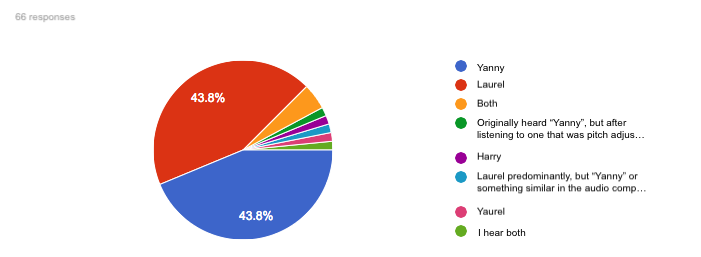
\includegraphics[width=2.34in,height=\textheight]{images/07_yl1.png}
\end{center}

\begin{center}
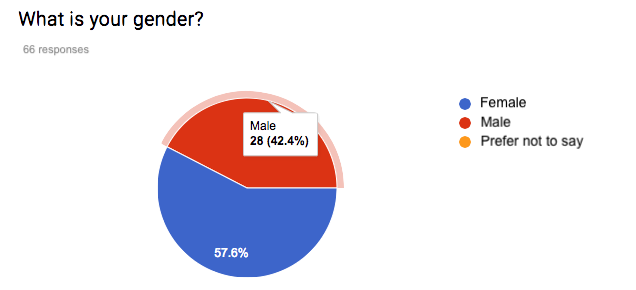
\includegraphics[width=2.12in,height=\textheight]{images/07_yl2.png}
\end{center}

\begin{center}
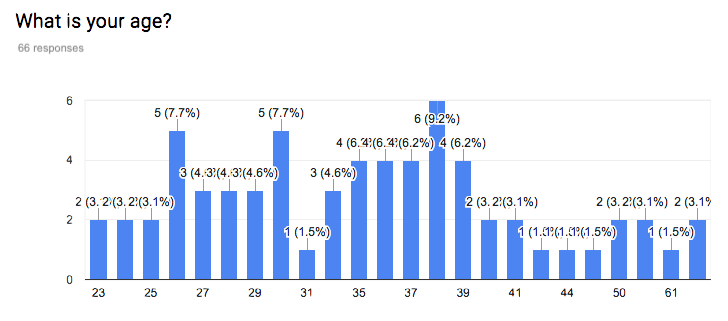
\includegraphics[width=2.43in,height=\textheight]{images/07_yl3.png}
\end{center}

The proportions hearing \texttt{Yanny} and \texttt{Laurel} are very
similar to each other, and there are some respondents who hear both or
even something completely different. This may be because people do not
listen to the audio file using the same device, something we couldn't
control for in the survey. Ignoring the responses other than
\texttt{Yanny} or \texttt{Laurel}, we have 53 observations.

\begin{tcolorbox}[enhanced jigsaw, leftrule=.75mm, title={Task 1}, rightrule=.15mm, opacitybacktitle=0.6, breakable, coltitle=black, toprule=.15mm, colback=white, toptitle=1mm, opacityback=0, colframe=quarto-callout-warning-color-frame, arc=.35mm, bottomtitle=1mm, colbacktitle=quarto-callout-warning-color!10!white, titlerule=0mm, bottomrule=.15mm, left=2mm]

Download the \texttt{yanny.csv} data and fit a logistic regression model
with \texttt{hear} as the binary response variable, and \texttt{age} and
\texttt{gender} as the explanatory variables. What are your findings?

See Solution

Load the data:

\begin{Shaded}
\begin{Highlighting}[]
\NormalTok{yanny }\OtherTok{\textless{}{-}} \FunctionTok{read.csv}\NormalTok{(}\StringTok{"yanny.csv"}\NormalTok{,}\AttributeTok{stringsAsFactors =}\NormalTok{ T)}
\NormalTok{yanny }\OtherTok{\textless{}{-}}\NormalTok{ yanny }\SpecialCharTok{\%\textgreater{}\%}
          \FunctionTok{select}\NormalTok{(hear, gender, age)}
\end{Highlighting}
\end{Shaded}

Exploratory Plots:

\begin{Shaded}
\begin{Highlighting}[]
\FunctionTok{ggplot}\NormalTok{(}\AttributeTok{data =}\NormalTok{ yanny, }\FunctionTok{aes}\NormalTok{(}\AttributeTok{x =}\NormalTok{ hear, }\AttributeTok{y =}\NormalTok{ age, }\AttributeTok{fill =}\NormalTok{ hear)) }\SpecialCharTok{+}
  \FunctionTok{geom\_boxplot}\NormalTok{() }\SpecialCharTok{+}
  \FunctionTok{labs}\NormalTok{(}\AttributeTok{x =} \StringTok{"What do you hear?"}\NormalTok{, }\AttributeTok{y =} \StringTok{"Age"}\NormalTok{) }\SpecialCharTok{+}
  \FunctionTok{theme}\NormalTok{(}\AttributeTok{legend.position =} \StringTok{"none"}\NormalTok{)}
\end{Highlighting}
\end{Shaded}

\begin{verbatim}
Warning: Removed 1 row containing non-finite outside the scale range
(`stat_boxplot()`).
\end{verbatim}

\begin{figure}[H]

{\centering 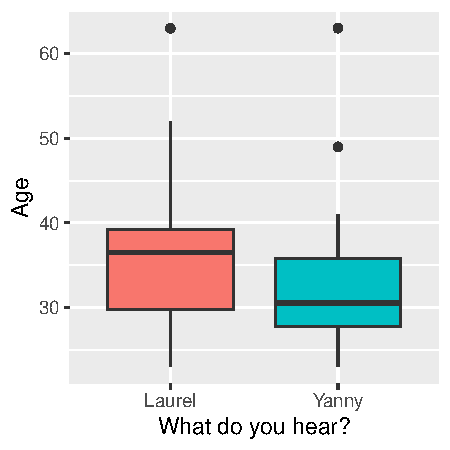
\includegraphics{about_files/figure-pdf/unnamed-chunk-3-1.pdf}

}

\caption{Hearing Yanny/Laurel by age.}

\end{figure}%

We see in the boxplot that the people who hear Yanny are, on average,
younger, however there is some overlap in the IQR's.

\begin{Shaded}
\begin{Highlighting}[]
\NormalTok{yanny }\SpecialCharTok{\%\textgreater{}\%}
  \FunctionTok{tabyl}\NormalTok{(gender, hear) }\SpecialCharTok{\%\textgreater{}\%}
  \FunctionTok{adorn\_percentages}\NormalTok{() }\SpecialCharTok{\%\textgreater{}\%}
  \FunctionTok{adorn\_pct\_formatting}\NormalTok{() }\SpecialCharTok{\%\textgreater{}\%}
  \FunctionTok{adorn\_ns}\NormalTok{() }\CommentTok{\# To show original counts}
\end{Highlighting}
\end{Shaded}

\begin{verbatim}
 gender     Laurel      Yanny
 Female 50.0% (14) 50.0                                                (14)
   Male 56.0% (14) 44.0                                                (11)
\end{verbatim}

\begin{Shaded}
\begin{Highlighting}[]
\FunctionTok{ggplot}\NormalTok{(}\AttributeTok{data =}\NormalTok{ yanny, }\FunctionTok{aes}\NormalTok{(}\AttributeTok{x =}\NormalTok{ hear, }\AttributeTok{group =}\NormalTok{ gender)) }\SpecialCharTok{+}
  \FunctionTok{geom\_bar}\NormalTok{(}\FunctionTok{aes}\NormalTok{(}\AttributeTok{y =}\NormalTok{ ..prop.., }\AttributeTok{fill =}\NormalTok{ gender),}
           \AttributeTok{stat =} \StringTok{"count"}\NormalTok{, }\AttributeTok{position =} \StringTok{"dodge"}\NormalTok{) }\SpecialCharTok{+}
  \FunctionTok{labs}\NormalTok{(}\AttributeTok{x =} \StringTok{"What do you hear?"}\NormalTok{, }\AttributeTok{y =} \StringTok{"Proportion"}\NormalTok{)}
\end{Highlighting}
\end{Shaded}

\begin{figure}[H]

{\centering 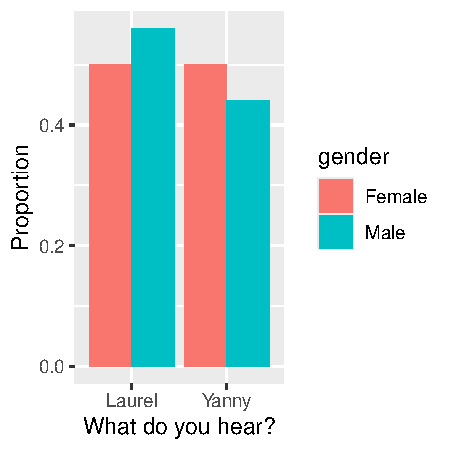
\includegraphics{about_files/figure-pdf/unnamed-chunk-5-1.pdf}

}

\caption{Barplot of what participants heard by gender.}

\end{figure}%

There is a slightly smaller proportion of men hearing \texttt{Yanny},
but the proportions are very similar overall.

\begin{Shaded}
\begin{Highlighting}[]
\NormalTok{mod.yanny }\OtherTok{\textless{}{-}} \FunctionTok{glm}\NormalTok{(hear }\SpecialCharTok{\textasciitilde{}}\NormalTok{ age }\SpecialCharTok{+}\NormalTok{ gender, }\AttributeTok{data =}\NormalTok{ yanny,}\AttributeTok{family=}\StringTok{"binomial"}\NormalTok{)}

\NormalTok{mod.yanny }\SpecialCharTok{\%\textgreater{}\%}
  \FunctionTok{tab\_model}\NormalTok{(}\AttributeTok{transform =} \ConstantTok{NULL}\NormalTok{)}
\end{Highlighting}
\end{Shaded}

\begin{longtable}[]{@{}cccc@{}}
\toprule\noalign{}
\endhead
\bottomrule\noalign{}
\endlastfoot
~ & \multicolumn{3}{c@{}}{%
hear} \\
Predictors & Log-Odds & CI & p \\
(Intercept) & 1.63 & -0.72~--~4.24 & 0.191 \\
age & -0.05 & -0.12~--~0.01 & 0.155 \\
gender {[}Male{]} & -0.21 & -1.34~--~0.91 & 0.717 \\
Observations & \multicolumn{3}{l@{}}{%
52} \\
R\textsuperscript{2} Tjur & \multicolumn{3}{l@{}}{%
0.045} \\
\end{longtable}

Notice that the coefficient of \texttt{age} is negative, suggesting that
older people are less likely to hear \texttt{Yanny}. However, the
coefficient of \texttt{age} is not significant (\(p\)-value of 0.16).
Still, if we wanted to use the estimated coefficient to quantify the
effect of \texttt{age}, we would need to look at exp(-0.05) = 0.95. This
suggests that for two people who differ by one year in age, the older
person's odds of hearing \texttt{Yanny} are 0.95 times those of the
younger person. If we want to look at a ten-year age difference then the
odds multiplier becomes exp(-0.05 * 10) = 0.6. Hence, for two people who
differ by 10 years in age, the older person's odds of hearing
\texttt{Yanny} are 0.6 times those of the younger person. Conversely,
the odds for a younger person of hearing \texttt{Yanny} would be
\texttt{exp(-0.05\ *\ 10)\^{}-1\ =\ 1.65} times the odds (64\% higher
odds) of hearing \texttt{Yanny} than 10 year older person.

\begin{Shaded}
\begin{Highlighting}[]
\FunctionTok{plot\_model}\NormalTok{(mod.yanny, }\AttributeTok{show.values =} \ConstantTok{TRUE}\NormalTok{,}
           \AttributeTok{title =} \StringTok{"Odds (Age)"}\NormalTok{, }\AttributeTok{show.p =} \ConstantTok{TRUE}\NormalTok{)}
\end{Highlighting}
\end{Shaded}

\begin{figure}[H]

{\centering 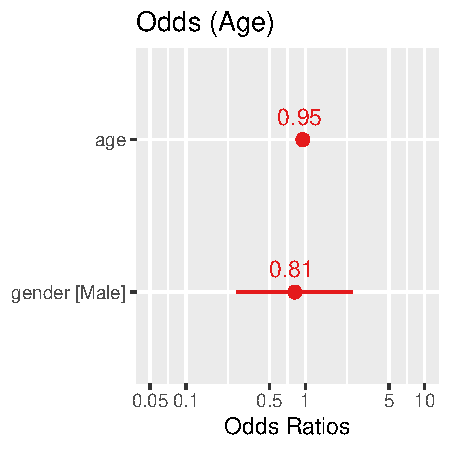
\includegraphics{about_files/figure-pdf/unnamed-chunk-7-1.pdf}

}

\caption{Odds of hearing yanny with age.}

\end{figure}%

\begin{Shaded}
\begin{Highlighting}[]
\FunctionTok{plot\_model}\NormalTok{(mod.yanny,}
           \AttributeTok{type =} \StringTok{"pred"}\NormalTok{, }
           \AttributeTok{terms =} \StringTok{"age"}\NormalTok{, }
           \AttributeTok{title =} \StringTok{""}\NormalTok{,}
           \AttributeTok{axis.title =} \FunctionTok{c}\NormalTok{(}\StringTok{"Age"}\NormalTok{, }\StringTok{"Probability of hearing Yanny"}\NormalTok{))}
\end{Highlighting}
\end{Shaded}

\begin{figure}[H]

{\centering 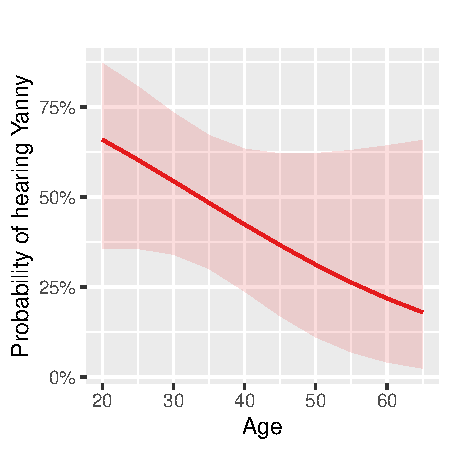
\includegraphics{about_files/figure-pdf/unnamed-chunk-8-1.pdf}

}

\caption{Probability of hearing Yanny with age.}

\end{figure}%

\end{tcolorbox}

\section{Case 2: Surviving the
Titanic}\label{case-2-surviving-the-titanic}

On 15th April 1912, during its maiden voyage, the
\href{https://en.wikipedia.org/wiki/RMS_Titanic}{Titanic} sank after
colliding with an iceberg, killing 1502 out of 2224 passengers and crew.
One of the reasons that the shipwreck led to such loss of life was that
there were not enough lifeboats for the passengers and crew. Although
there was some element of luck involved in surviving the sinking, some
groups of people were more likely to survive than others, such as women,
children, and the upper-class.

\begin{tcolorbox}[enhanced jigsaw, leftrule=.75mm, title={Task 2}, rightrule=.15mm, opacitybacktitle=0.6, breakable, coltitle=black, toprule=.15mm, colback=white, toptitle=1mm, opacityback=0, colframe=quarto-callout-warning-color-frame, arc=.35mm, bottomtitle=1mm, colbacktitle=quarto-callout-warning-color!10!white, titlerule=0mm, bottomrule=.15mm, left=2mm]

Download the data (\texttt{titanic.csv)} for \(n = 891\) passengers
aboard the Titanic and fit a logistic regression model with
\texttt{survived} as the binary response variable, and \texttt{age},
\texttt{gender}, and \texttt{passenger.class} as the explanatory
variables. What are your findings?

See Solution

Load the data

\begin{Shaded}
\begin{Highlighting}[]
\NormalTok{titanic }\OtherTok{\textless{}{-}} \FunctionTok{read.csv}\NormalTok{(}\StringTok{"titanic.csv"}\NormalTok{,}\AttributeTok{stringsAsFactors =}\NormalTok{ T)}
\NormalTok{titanic }\OtherTok{\textless{}{-}}\NormalTok{ titanic }\SpecialCharTok{\%\textgreater{}\%}
          \FunctionTok{select}\NormalTok{(survived, age, gender, passenger.class) }\SpecialCharTok{\%\textgreater{}\%}
  \FunctionTok{mutate}\NormalTok{(}\AttributeTok{passenger.class =} \FunctionTok{as.factor}\NormalTok{(passenger.class),}
         \AttributeTok{survived\_fct =} \FunctionTok{as.factor}\NormalTok{(survived))}
\FunctionTok{levels}\NormalTok{(titanic}\SpecialCharTok{$}\NormalTok{survived\_fct) }\OtherTok{\textless{}{-}} \FunctionTok{c}\NormalTok{(}\StringTok{"Died"}\NormalTok{, }\StringTok{"Survived"}\NormalTok{)}
\end{Highlighting}
\end{Shaded}

\begin{Shaded}
\begin{Highlighting}[]
\FunctionTok{ggplot}\NormalTok{(}\AttributeTok{data =}\NormalTok{ titanic, }\FunctionTok{aes}\NormalTok{(}\AttributeTok{x =}\NormalTok{ survived\_fct, }\AttributeTok{y =}\NormalTok{ age, }\AttributeTok{fill =}\NormalTok{ survived\_fct)) }\SpecialCharTok{+}
  \FunctionTok{geom\_boxplot}\NormalTok{() }\SpecialCharTok{+}
  \FunctionTok{labs}\NormalTok{(}\AttributeTok{x =} \StringTok{"Survived the Titanic?"}\NormalTok{, }\AttributeTok{y =} \StringTok{"Age"}\NormalTok{) }\SpecialCharTok{+}
  \FunctionTok{theme}\NormalTok{(}\AttributeTok{legend.position =} \StringTok{"none"}\NormalTok{)}
\end{Highlighting}
\end{Shaded}

\begin{figure}[H]

{\centering 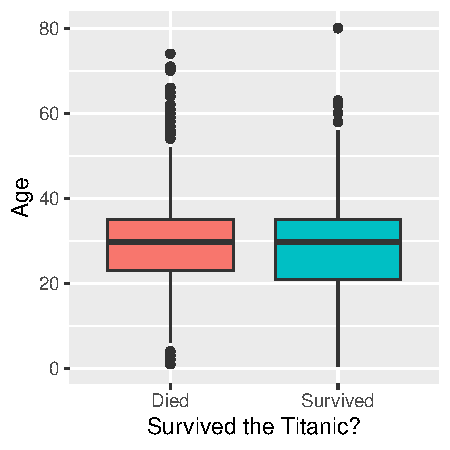
\includegraphics{about_files/figure-pdf/unnamed-chunk-10-1.pdf}

}

\caption{Titanic passenger age by survival.}

\end{figure}%

We see in the boxplot that there is very little difference in the age of
passengers who died or survived the sinking of the Titanic.

\begin{Shaded}
\begin{Highlighting}[]
\NormalTok{titanic }\SpecialCharTok{\%\textgreater{}\%}
  \FunctionTok{tabyl}\NormalTok{(gender, survived\_fct) }\SpecialCharTok{\%\textgreater{}\%}
  \FunctionTok{adorn\_percentages}\NormalTok{() }\SpecialCharTok{\%\textgreater{}\%}
  \FunctionTok{adorn\_pct\_formatting}\NormalTok{() }\SpecialCharTok{\%\textgreater{}\%}
  \FunctionTok{adorn\_ns}\NormalTok{() }\CommentTok{\# To show original counts}
\end{Highlighting}
\end{Shaded}

\begin{verbatim}
 gender        Died    Survived
 female 25.8%  (81) 74.2                                              (233)
   male 81.1% (468) 18.9                                              (109)
\end{verbatim}

\begin{Shaded}
\begin{Highlighting}[]
\FunctionTok{ggplot}\NormalTok{(}\AttributeTok{data =}\NormalTok{ titanic, }\FunctionTok{aes}\NormalTok{(}\AttributeTok{x =}\NormalTok{ survived\_fct, }\AttributeTok{group =}\NormalTok{ gender)) }\SpecialCharTok{+}
  \FunctionTok{geom\_bar}\NormalTok{(}\FunctionTok{aes}\NormalTok{(}\AttributeTok{y =}\NormalTok{ ..prop.., }\AttributeTok{fill =}\NormalTok{ gender), }\AttributeTok{stat =} \StringTok{"count"}\NormalTok{, }\AttributeTok{position =} \StringTok{"dodge"}\NormalTok{) }\SpecialCharTok{+}
  \FunctionTok{labs}\NormalTok{(}\AttributeTok{x =} \StringTok{"Survived the Titanic?"}\NormalTok{, }\AttributeTok{y =} \StringTok{"Proportion"}\NormalTok{)}
\end{Highlighting}
\end{Shaded}

\begin{figure}[H]

{\centering 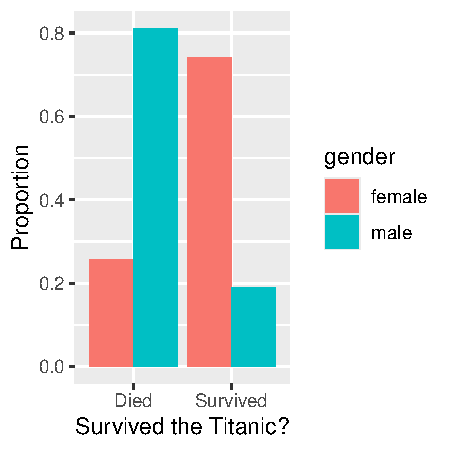
\includegraphics{about_files/figure-pdf/unnamed-chunk-12-1.pdf}

}

\caption{Barplot of passenger survival by gender.}

\end{figure}%

There is a clear pattern here with the proportion surviving much higher
for females than for males.

\begin{Shaded}
\begin{Highlighting}[]
\NormalTok{titanic }\SpecialCharTok{\%\textgreater{}\%}
  \FunctionTok{tabyl}\NormalTok{(passenger.class, survived) }\SpecialCharTok{\%\textgreater{}\%}
  \FunctionTok{adorn\_percentages}\NormalTok{() }\SpecialCharTok{\%\textgreater{}\%}
  \FunctionTok{adorn\_pct\_formatting}\NormalTok{() }\SpecialCharTok{\%\textgreater{}\%}
  \FunctionTok{adorn\_ns}\NormalTok{() }\CommentTok{\# To show original counts}
\end{Highlighting}
\end{Shaded}

\begin{verbatim}
 passenger.class           0           1
               1 37.0%  (80) 63.0                                     (136)
               2 52.7%  (97) 47.3%  (87)
               3 75.8% (372) 24.2                                     (119)
\end{verbatim}

\begin{Shaded}
\begin{Highlighting}[]
\FunctionTok{ggplot}\NormalTok{(}\AttributeTok{data =}\NormalTok{ titanic, }\FunctionTok{aes}\NormalTok{(}\AttributeTok{x =}\NormalTok{ survived\_fct, }\AttributeTok{group =}\NormalTok{ passenger.class)) }\SpecialCharTok{+}
  \FunctionTok{geom\_bar}\NormalTok{(}\FunctionTok{aes}\NormalTok{(}\AttributeTok{y =}\NormalTok{ ..prop.., }\AttributeTok{fill =}\NormalTok{ passenger.class),}
            \AttributeTok{stat =} \StringTok{"count"}\NormalTok{, }\AttributeTok{position =} \StringTok{"dodge"}\NormalTok{) }\SpecialCharTok{+}
  \FunctionTok{labs}\NormalTok{(}\AttributeTok{x =} \StringTok{"Survived the Titanic?"}\NormalTok{, }\AttributeTok{y =} \StringTok{"Proportion"}\NormalTok{)}
\end{Highlighting}
\end{Shaded}

\begin{figure}[H]

{\centering 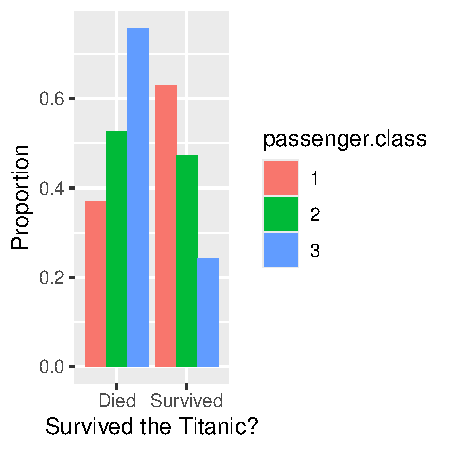
\includegraphics{about_files/figure-pdf/unnamed-chunk-14-1.pdf}

}

\caption{Barplot of passenger survival by gender.}

\end{figure}%

The largest group of passengers who died were third class passengers,
while among those who survived the largest group was first class
passengers.

Now we focus on the event \(\text{Probability}(\text{Survival = 1})\).
We will as our response the binary variable \texttt{survived} which
takes the value of 1 if the i\emph{th} passenger survived and zero
othewise.

\begin{Shaded}
\begin{Highlighting}[]
\NormalTok{mod.titanic }\OtherTok{\textless{}{-}} \FunctionTok{glm}\NormalTok{(survived }\SpecialCharTok{\textasciitilde{}}\NormalTok{ gender }\SpecialCharTok{+}\NormalTok{ passenger.class }\SpecialCharTok{+}\NormalTok{ age, }\AttributeTok{data =}\NormalTok{ titanic) }
\NormalTok{mod.titanic }\SpecialCharTok{\%\textgreater{}\%}
  \FunctionTok{tab\_model}\NormalTok{(}\AttributeTok{transform =} \ConstantTok{NULL}\NormalTok{)}
\end{Highlighting}
\end{Shaded}

\begin{longtable}[]{@{}cccc@{}}
\toprule\noalign{}
\endhead
\bottomrule\noalign{}
\endlastfoot
~ & \multicolumn{3}{c@{}}{%
survived} \\
Predictors & Estimates & CI & p \\
(Intercept) & 1.10 & 1.00~--~1.19 & \textbf{\textless0.001} \\
gender {[}male{]} & -0.50 & -0.55~--~-0.45 & \textbf{\textless0.001} \\
passenger class {[}2{]} & -0.18 & -0.26~--~-0.10 &
\textbf{\textless0.001} \\
passenger class {[}3{]} & -0.37 & -0.44~--~-0.30 &
\textbf{\textless0.001} \\
age & -0.01 & -0.01~--~-0.00 & \textbf{\textless0.001} \\
Observations & \multicolumn{3}{l@{}}{%
891} \\
R\textsuperscript{2} & \multicolumn{3}{l@{}}{%
0.383} \\
\end{longtable}

We see that the coefficient for males (\texttt{gendermale}) is negative,
indicating a lower chance of survival for male passengers. Similarly,
the coefficients for second (\texttt{passenger.class2}) and third
(\texttt{passenger.class3}) class passengers are negative, with the
magnitude of the third class coefficient larger than that of the second
class coefficient. This suggests that second class passengers chances of
survival were worse in comparison with first class passengers, and that
third class passengers chances of survival were even worse. Finally the
\texttt{age} coefficient is negative, suggesting that older people were
less likely to survive.

\begin{Shaded}
\begin{Highlighting}[]
\FunctionTok{plot\_model}\NormalTok{(mod.titanic,}
           \AttributeTok{transform =} \StringTok{"exp"}\NormalTok{,}
           \AttributeTok{show.values =} \ConstantTok{TRUE}\NormalTok{,}
           \AttributeTok{title =} \StringTok{""}\NormalTok{,}
           \AttributeTok{show.p =} \ConstantTok{FALSE}\NormalTok{, }
           \AttributeTok{value.offset =} \FloatTok{0.25}\NormalTok{)}
\end{Highlighting}
\end{Shaded}

\begin{figure}[H]

{\centering 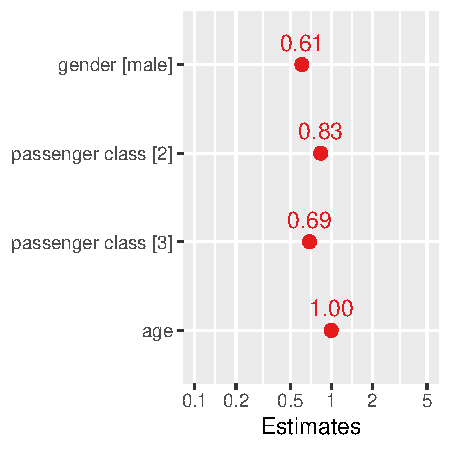
\includegraphics{about_files/figure-pdf/unnamed-chunk-16-1.pdf}

}

\caption{Odds of surviving the sinking of the Titanic.}

\end{figure}%

We interpret the odds ratios as follows: men's odds of survival were
0.61 times those of women, third class passengers' odds of survival were
0.7 times those of first class passengers, and second class passengers'
odds of survival were 0.83 times those of first class passengers.
Finally, for each year increase in the passenger's age, their odds of
survival decrease (by a factor of 0.99).

\end{tcolorbox}



\end{document}
